\section{Anomalous Test Case Result with IBM Compiler}
%=====================================================
\label{app:busted_ibm_compiler_results}
This section briefly details the results for the LBLRTM v11.3 user-defined atmosphere test case when the IBM AIX xlf95 v10.1.0000.0002 compiler is used (henceforth referred to as v10.1.0.2) . You can find out the version of your IBM compiler via the \texttt{-qversion} switch:
\begin{verbatim}
  $ xlf95 -qversion
  IBM XL Fortran Enterprise Edition V10.1 for AIX
  Version: 10.01.0000.0002\end{verbatim}

The anomalous LBLRTM v11.3 results only occur for this compiler version and only for the double precision build -- the single precision build does not appear to have any problem. Additionally, the problem also only occurs for the user-defined atmosphere test case; the built-in atmosphere test case produces expected results for all builds using the v10.1.0.2 AIX compiler. Thus, it is thought that the anomalous results stem from some sort of interaction between the double precision build and the use of the \texttt{SCAN} options - in this particular case the \texttt{FFTSCN} option, but similar anomalous results have been seen when the \texttt{SCNMRG} option has been used.
 
\begin{figure}[htp]
  \centering
  \qquad\sffamily\textbf{Verification Example: Built-in Atmosphere Upwelling}\\
  \qquad\sffamily\textbf{IBM AIX xlf95 v10.1.0.2 compiler; double precision build}\\
  \qquad\textsf{LBLRTM v11.3 brightness temperature difference using AER TAPE3}\\
  \includegraphics[bb=80 403 534 558,clip,scale=1.0]{graphics/run_example_user_defined_upwelling/ibm/dbl-busted-dt.eps}
  \qquad\textsf{LBLRTM v11.3 brightness temperature spectra using AER TAPE3}\\
  \includegraphics[bb=80 403 534 558,clip,scale=1.0]{graphics/run_example_user_defined_upwelling/ibm/dbl-busted-t.eps}
  \caption{Comparison of the AER-supplied \texttt{TAPE27\_ex} output to the locally generated \texttt{TAPE27} output for the \textsl{double precision} version of LBLRTM v11.3 using the IBM AIX xlf 95 v10.1.0.2 compiler. The AER-supplied big-endian \texttt{TAPE3} spectroscopic datafile was used. \mbox{\textbf{(Upper Panel)} Brightness} temperature differences. \mbox{\textbf{(Lower Panel)} Brightness} temperature spectra. The locally generated result using the v10.1.0.2 compiler is clearly incorrect.}
  \label{fig:run_example_user_defined_atm_upwelling-dbl-ibm_busted}
\end{figure}

